\documentclass[oneside, 11pt]{article}

\usepackage[T1]{fontenc}
\usepackage[utf8]{inputenc}
\usepackage[dutch]{babel}

\usepackage{fouriernc}
\usepackage[detect-all, load-configurations=binary,
            separate-uncertainty=true, per-mode=symbol,
            retain-explicit-plus, range-phrase={ tot }]{siunitx}

\usepackage{setspace}
\setstretch{1.2}

\setlength{\parskip}{\smallskipamount}
\setlength{\parindent}{0pt}

\usepackage{geometry}
\geometry{marginparwidth=0.5cm, verbose, a4paper, tmargin=3cm, bmargin=3cm, lmargin=2cm, rmargin=2cm}

\usepackage{float}

\usepackage[fleqn]{amsmath}
\numberwithin{equation}{section}
\numberwithin{figure}{section}

\usepackage{graphicx}
\graphicspath{{Figures/}}
\usepackage{subfig}

\usepackage{tikz}
\usetikzlibrary{plotmarks}

\usepackage{fancyhdr}
\pagestyle{fancy}
\fancyhf{}
\rhead{\thepage}
\renewcommand{\footrulewidth}{0pt}
\renewcommand{\headrulewidth}{0pt}

\usepackage{relsize}
\usepackage{xspace}
\usepackage{url}

\newcommand{\figref}[1]{Figuur~\ref{#1}}

\newcommand{\hisparc}{\textsmaller{HiSPARC}\xspace}
\newcommand{\kascade}{\textsmaller{KASCADE}\xspace}
\newcommand{\sapphire}{\textsmaller{SAPPHiRE}\xspace}
\newcommand{\jsparc}{\textsmaller{jSparc}\xspace}
\newcommand{\hdf}{\textsmaller{HDF5}\xspace}
\newcommand{\aires}{\textsmaller{AIRES}\xspace}
\newcommand{\csv}{\textsmaller{CSV}\xspace}
\newcommand{\python}{\textsmaller{PYTHON}\xspace}
\newcommand{\corsika}{\textsmaller{CORSIKA}\xspace}
\newcommand{\labview}{\textsmaller{LabVIEW}\xspace}
\newcommand{\daq}{\textsmaller{DAQ}\xspace}
\newcommand{\adc}{\textsmaller{ADC}\xspace}
\newcommand{\adcs}{\textsmaller{ADC}s\xspace}
\newcommand{\Adcs}{A\textsmaller{DC}s\xspace}
\newcommand{\hi}{\textsc{h i}\xspace}
\newcommand{\hii}{\textsc{h ii}\xspace}
\newcommand{\mip}{\textsmaller{MIP}\xspace}
\newcommand{\hisparcii}{\textsmaller{HiSPARC II}\xspace}
\newcommand{\hisparciii}{\textsmaller{HiSPARC III}\xspace}
\newcommand{\pmt}{\textsmaller{PMT}\xspace}
\newcommand{\pmts}{\textsmaller{PMT}s\xspace}

\DeclareSIUnit{\electronvolt}{\ensuremath{\mathrm{e\!\!\:V}}}

\DeclareSIUnit{\unitsigma}{\ensuremath{\sigma}}
\DeclareSIUnit{\mip}{\textsmaller{MIP}}
\DeclareSIUnit{\adc}{\textsmaller{ADC}}

\DeclareSIUnit{\gauss}{G}
\DeclareSIUnit{\parsec}{pc}
\DeclareSIUnit{\year}{yr}



\title{Werken met Python Notebooks}
\author{N.G. Schultheiss}
\docpython{2}{WP}
\version{1.0}

\begin{document}

\maketitle

\section{Inleiding}

Python wordt veel gebruikt om meetgegevens te verwerken en simulaties van meetsystemen en natuurkundige 
processen door te rekenen. De taal is object geor\"\i enteerd en gebruikt variabelen net iets anders dan andere 
talen.

Een notebook is een interactieve leeromgeving voor Python. In deze leeromgeving kunnen de instructies na elkaar worden 
uitgevoerd. Zonder update-problemen werken de opdrachten in \'{e}\'{e}n keer. Verder hebben notebooks het voordeel 
dat de opdrachten aan te passen zijn. Eventueel kunnen zelfs cellen met nieuwe opdrachten worden toegevoegd. Met 
enig begrip van python is het dus mogelijk om een notebook aan te passen aan de eigen wensen. 

Een nadeel is dat de opdrachten door elkaar uit te voeren zijn, bijvoorbeeld eerst de derde en dan de eerste opdracht. Dit leidt tot problemen. 

Op \url{http://docs.hisparc.nl/infopakket/} zijn notebooks te vinden voor\footnote{Het ophalen van notebooks is beschreven in `Notebook installatie'. Documentatie van overige \hisparc software is te vinden op \url{http://docs.hisparc.nl/}.}:
\begin{itemize}
\item Het ophalen van meetgegegevens.
\item Het ophalen van stationsgegevens.
\item Het verwerken van de opgehaalde gegevens
\end{itemize}

\section{De notebook server}

Notebooks worden in de computer op een lokale server bijgehouden\footnote{De server gebruikt poort 8888, deze moet in de firewall dus open staan.}. De informatie op deze server is op de computer via een browser, zoals firefox of chrome, te bekijken. 

\begin{figure}[H]
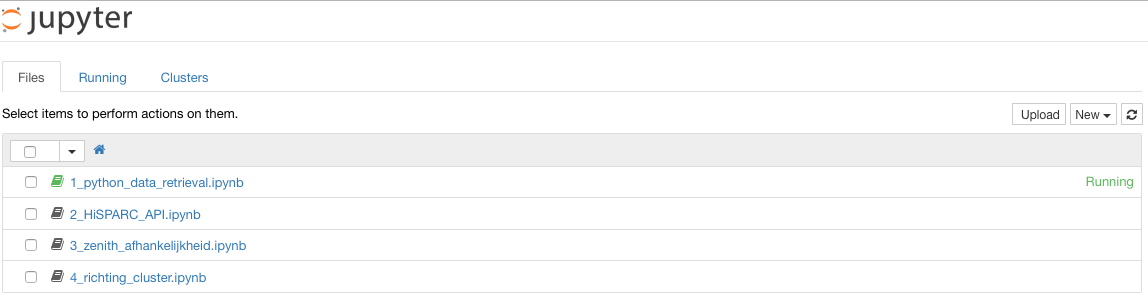
\includegraphics[width=16cm]{home.png}
\caption{Het `Home' tabblad. Er draait een virtuele computer voor het tabblad `1\_python\_data\_retrieval'. Dit is te zien
aan het groene notebook icoontje en `Running' achterin de regel.}
\end{figure}

Op de home-pagina kunnen we de diverse notebooks vinden. Verder kunnen we de programma's, om de notebooks op de lokale server te laten werken, aansturen.

\begin{figure}[H]
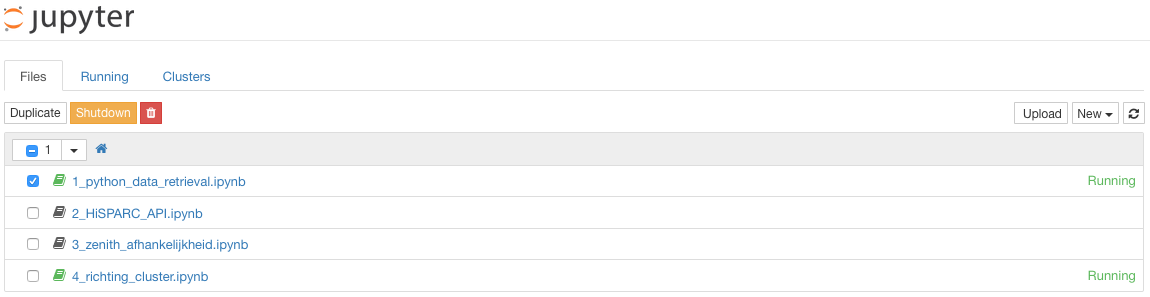
\includegraphics[width=16cm]{home_select.png}
\caption{`Python data retrieval' is in het `Home'-tabblad geselecteerd. De selectie is nu te dupliceren, af te sluiten of weg te gooien.}
\end{figure}

In de home-pagina werkt `1\_python\_data\_retrieval' als een link. Als we er op klikken opent een nieuw tabblad.

\begin{figure}[H]

\includegraphics[width=16cm]{header.png}
\caption{In de kop van `Python data retrieval' zijn twee menulagen te zien. Een rij met termen en een rij met pictogrammen.}
\end{figure}

Als we met een notebook gaan werken, verdient het aanbeveling om de kernel opnieuw te starten. Klik op 'Kernel', er verschijnt een pop-up menu. Kies `Restart' en alle vorige bewerkingen worden vergeten. Klik hierna op `Cell', kies `All Output' en daarna `Clear'. Het noteboot is hierna schoon.

Het is mogelijk om een duplicaat (kopie) van een programma te maken. De oude notebook blijft bestaan en de nieuwe notebook is aan te passen. 

Het pictogram waarin een pijltje naar rechts afgebeeld staat, werkt als `Shift-Enter' toets. Het geselecteerde commando wordt uitgevoerd. Als het commando wordt bewerkt is voor dit blok een sterretje te zien. Als het commando is uitgevoerd, wordt het sterretje vervangen door een volgnummer.

\section{Notebooks}

Notebooks hebben een afwisselende structuur. Er zijn blokken uitleg en blokken waarin de programmeer code kan worden onderzocht of aangepast. Het doorwerken en aanpassen van de blokken aan eigen idee\"{e}n is te beschouwen als een introductie van het programmeren. Ieder notebook is te beschouwen als een programmeer-practicum van ongeveer \"{e}\"{e}n lesuur.
 
Met `Python data retrieval' kunnen de meetgegevens van een station worden opgehaald. De gegevens worden opgeslagen in `.h5' formaat. Dit bestand heeft een inwendige structuur. Uitgelegd wordt hoe een enkel gegeven uit de berg informatie te halen is. 

Naast de meetgegevens is het noodzakelijk om informatie over het meetnetwerk te verzamelen. De eigenschappen van een station zijn op te halen met `HiSPARC-API'.  

Nadat onderzocht is hoe de meetgegevens en stationsgegevens opgehaald kunnen worden, is het mogelijk om te onderzoeken \textit{wat} er gemeten is. Een eenvoudige reconstructie wordt uitgelegd in `Zenith-afhankelijkheid van een station'. Als uitvoer wordt een lijst met hoeken gegenereerd.

Uiteindelijk willen we grafieken kunnen maken. In `Richtingreconstructie met een cluster' wordt uitgelegd hoe deze gegevens in een scatterplot en een histogram te verwerken zijn.

\section{Vervolg}

De door \hisparc gepubliceerde notebooks geven een aardige start voor het verwerken van gegevens met \python.
Eventueel is na deze start een eigen notebook te maken, dit kan door op de `New' knop rechts boven in het tabblad `Home' te
klikken. Het nieuwe tabblad heeft dezelfde kop, middenin is een pulldown menu te zien. De notebooks gebruiken de opties:

\begin{itemize}
\item Code: Hier wordt een code-cel mee gemaakt.
\item Markdown: Hier is verklarende tekst te typen. Deze voldoet aan het Markdown protocol. Dubbelklikken op een Markdown-cel
toont de broncode van de cel. `Shift + Enter' laat de cel met layout weer zien.
\end{itemize}

Bij het schrijven van een eigen notebook kunnen de volgende trefwoorden als bij het googelen nuttig zijn:

\python, NumPy, SciPy, matplotlib, list, array, Markdown, \hisparc, \sapphire, GitHub.

Internet is groot en beantwoordt veel vragen. Kritisch denken blijft van belang.

Na afloop wordt de `Jupyter Notebook' server afgesloten door
het eerste terminal-venster te selecteren en op `Control - C' te drukken.

\end{document}
